\subsection{Oscillating Conveyor Belt}

This test illustrates artifacts in the strongly coupled SAP and Similar
approximations. A $1 \text{ kg}$ box with $5\text{ cm}$ sides is placed on a
conveyor belt oscillating at $1 \text{ Hz}$ with $0.2 \text{ m}$ amplitude (Fig.
\ref{fig:belt_shematic}). Friction is $\mu=0.7$. Even though dissipation models
are different, using $d=500 \text{ s/m}$ for Similar and Lagged and
$\tau_d=10^{-3} \text{ s}$ for SAP yields comparable dissipation.

\begin{figure}[!h]
    \centering
    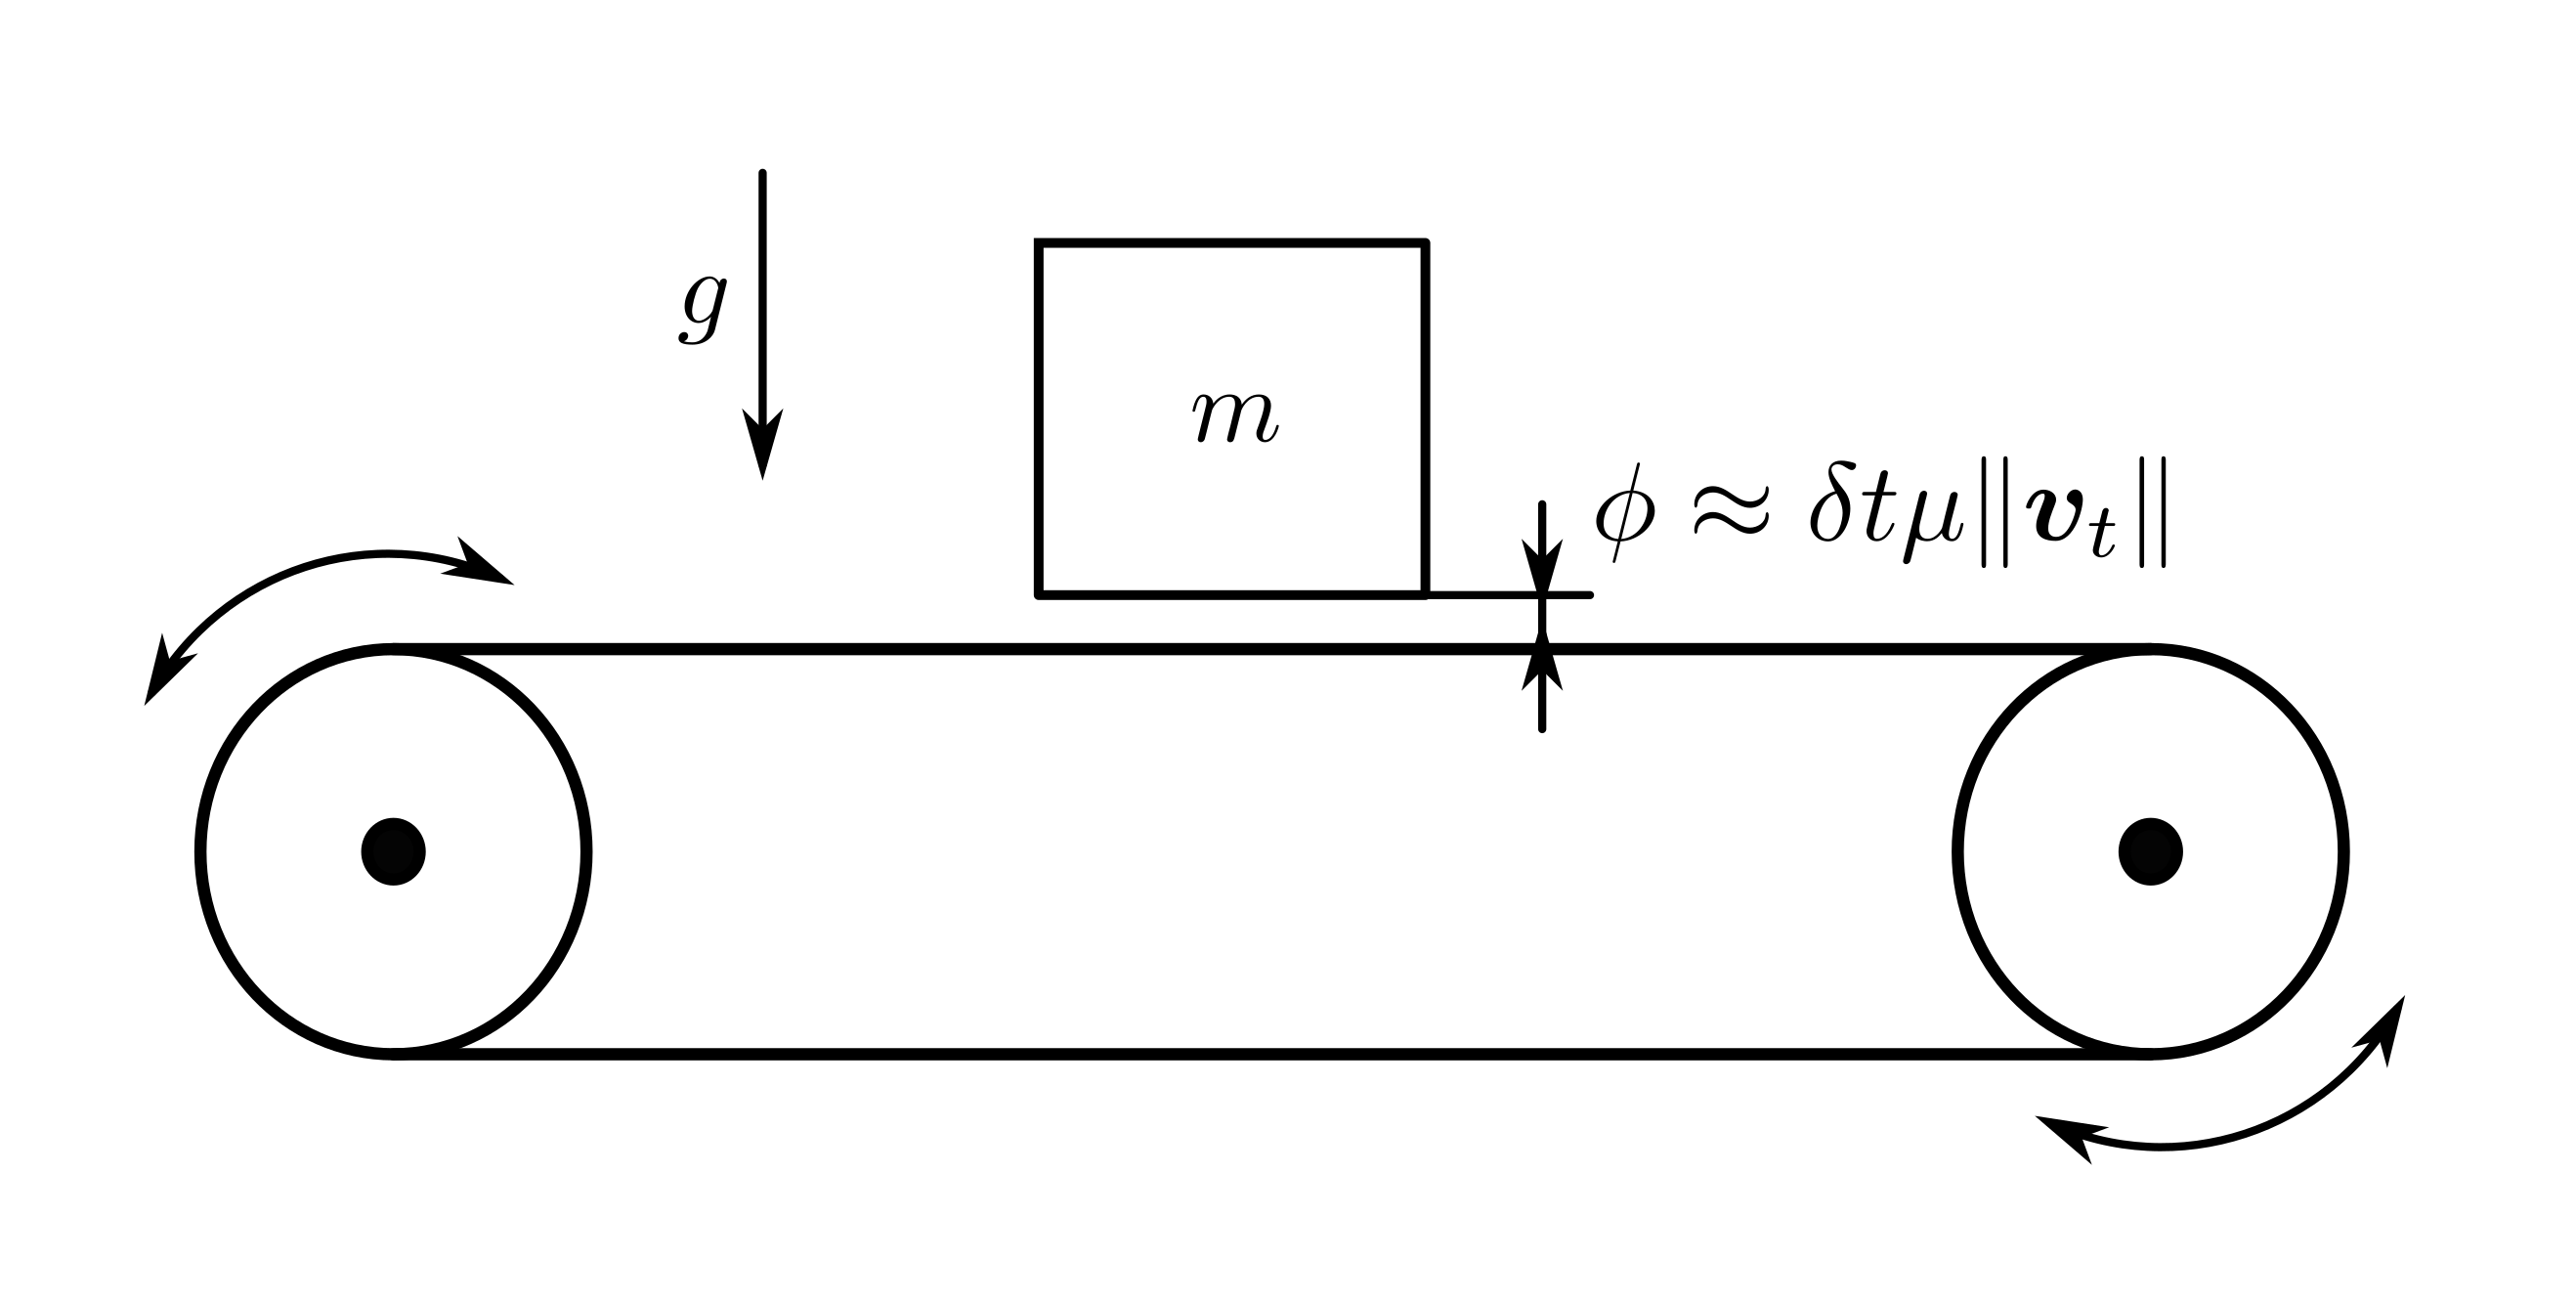
\includegraphics[width=0.8\columnwidth]{figures/TestCases/Belt/belt_schematics.png}
    \caption{Oscillating Conveyor Belt. SAP and Similar introduce artificial
    \emph{gliding} during slip phases (Section \ref{sec:gliding_artifact}).}
    \label{fig:belt_shematic}
\end{figure}

Figure \ref{fig:belt_contact_velocity_and_force} shows contact velocity and
force computed using $\delta t=0.01\text{ s}$. Contact between the box and belt
transitions back and forth between stiction and sliding. The Lagged
approximation predicts no vertical motion, with the normal force balancing the
box's weight as expected. However, SAP and Similar models show artifacts in the
normal direction during sliding, with non-zero normal velocity due to the
\emph{gliding} artifact, which disappears in stiction. Additionally, we observe
spurious transients in the normal force during sliding --- as slip speed changes
so does \emph{gliding}, causing vertical acceleration and thus normal force
fluctuations. Finally, SAP and Similar introduce normal force spikes
during the abrupt transition from sliding to stiction, when gliding vanishes
causing a sudden normal velocity change (Fig.
\ref{fig:belt_contact_velocity_and_force}).

\begin{figure}[!h]
    \centering
    %trim={<left> <lower> <right> <upper>}
    \adjincludegraphics[width=0.49\columnwidth,trim={0 0 {0.05\width} 0},clip]{figures/TestCases/Belt/contact_velocity_dt0p01.png}
    \adjincludegraphics[width=0.49\columnwidth,trim={0 0 {0.05\width} 0},clip]{figures/TestCases/Belt/contact_force_dt0p01.png}
    \caption{\label{fig:belt_contact_velocity_and_force} Contact velocity (left)
    and force (right). $\delta t=0.01\text{ s}$.}
\end{figure}

Figure \ref{fig:bel_convergence_position} shows a convergence study with step
sizes $\delta t \in \{2\times10^{-3}, 10^{-2}, 5\times10^{-2}\}$. Both Lagged
and Similar exhibit first order convergence, as expected, though the artifacts
introduced by Similar (Fig. \ref{fig:belt_contact_velocity_and_force}), cause
higher errors than Lagged. Finally, SAP's error plateaus at the smallest time
step due to model inconsistency, where the term $\tau_d\mu\Vert\vf{v}_t\Vert$ in
\eqref{eq:sap_gliding_offset} does not vanish as time step decreases.

\begin{figure}[!h]
    \centering
    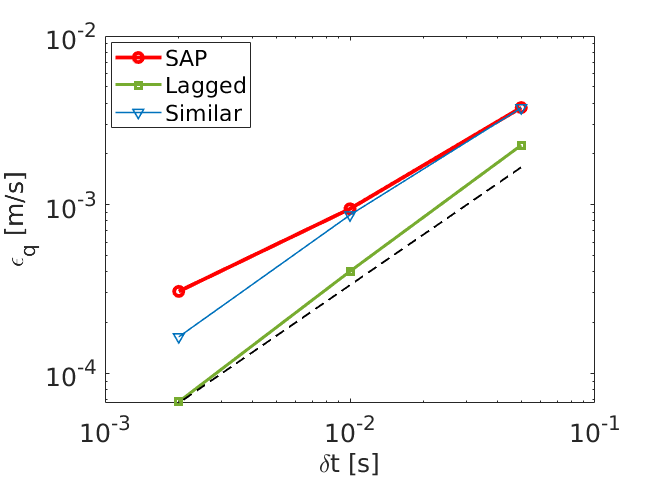
\includegraphics[width=0.8\columnwidth]{figures/TestCases/Belt/convergence_position.png}
    \caption{Convergence of the box trajectory with time step size. The dashed line is a reference for first order convergence.}
    \label{fig:bel_convergence_position}
\end{figure}
